\chapter{The Large Hadron Collider}
\label{capitolo_2}
The Large Hadron Collider (LHC) is the largest proton and heavy ions accelerator and collider ever built. It is designed to overcome the performances of the old kinds of accelerators, like Tevatron $\text{p}\bar{\text{p}}$ collider at Fermilab and the Lep $\text{e}^+\text{e}^-$ collider at Cern. The LHC was thought and designed to reach center-of-mass energies in order of 14 TeV with an instantaneous luminosity of $10^{34} \text{cm}^{-2}\text{s}^{-1}$ in proton-proton collisions. After some relevant technical issues which caused the reduction of the collisions energy in the early years since the switching on, at the state of art the accelerator works at its best performances.
\\\\
The idea of colliding proton instead of electrons is due to some physical constrains. Accelerating electrons in a circular path implies a huge amount of radiative energy losses. A charged particle in fact, if circularly accelerated, loses energy according to the relation\cite{jackson_classical_1999}
\begin{equation}
\frac{dE}{dt} \propto \frac{E^4}{m^4}
\end{equation}
where $E$ is the energy of the particle and $m$ is the mass. It is evident how the energy losses will be smaller for high masses and comparing the values for a proton and an electron, it turns up that in order to accelerate the latter to the same energy of a proton you have to compensate for an energy loss which is $(m_p / m_e) \sim 10^{13}$ higher.
\\\\
The draw back is that protons, unlike the electrons, are not elementary particles, but they are composed of partons and all of them will produce a lot of low-energy interactions, called \emph{underlying event}, that will interfere with the signal.

\section{The acceleration chain and LHC structure}
The LHC collider consists of a 27-kilometre ring of superconducting magnets and accelerates particles at energies up to the nominal value of 14 TeV in the center of mass through several stages \cite{Bruning}.
\\
For protons, the accelerator chain is composed of four stages, usefull to allow the particles rising the energy scale and focus the beams to increase the luminosity:
\begin{itemize}
\item a Linear Accelerator (LINAC) handles the very first part of the acceleration process, boosting the particles up to 50 MeV using Radio Frequency Quadrupoles (RFQ) and focusing quadrupole magnets;
\item the  Proton Synchrotron Booster, a circular accelerator consisting of four superimposed synchrotron rings, keeps on accelerating protons up to energies of 1.4 GeV;
\item the Proton Synchrotron (PS), a single synchrotron ring with a circumference of approximately 600 m, is where the protons reach an energy of 25 GeV;
\item the Super Proton Synchrotron (SPS), the upgraded model of the Proton Synchrotron with a  circumference of around 7 km, is the last link in the acceleration chain before the injection and speeds up the particles to 450 GeV.
\end{itemize} 
\begin{figure}[t]
\centering
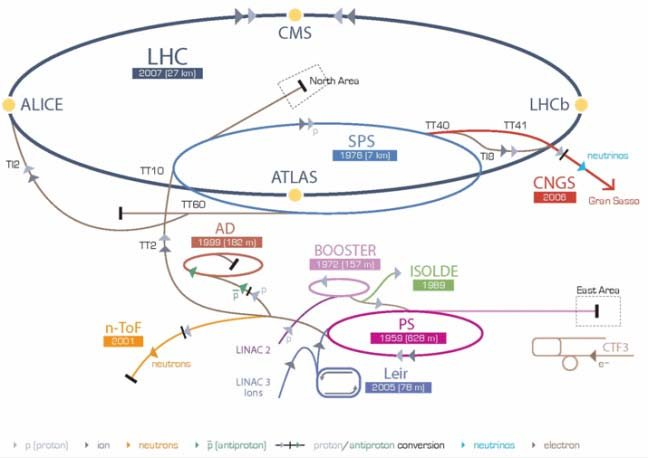
\includegraphics[scale=0.35]{CERN-accelerator-complex.jpg}
\caption{Accelerator complex at CERN}
\end{figure}
After the transition in the acceleration chain, protons are injected into LHC and they finally reach the nominal energy of $\sqrt{s}/2$. The beams travel in opposite directions in separate beam pipes, two ultra-high vacuum tubes, and are bended in the circular trajectory by a strong magnetic field mantained by superconducting deflecting dipole magnets, which operate at temperature of 1.9 K and produce a field of about 8.4 Tesla at a current of 11,700 A. The beam focusing relies on 392 quadrupole magnets acting on horizontal or vertical plane, depending on their polarity.
\\
The magnets are disposed along the ring in a modular layout, where each module is composed of six dipole magnets and two quadrupole magnets with opposite polarity. In order to fix the field non uniformities and so guarantee the stability of the two colliding beams, higher order magnets are installed at the end of the dipoles.
\\
At its full intensity, each proton beam is made of 2808 bunches of $10^{11}$ protons each and and collide with each other at four different interaction points where the main experiments are sited.
\vspace{0.3cm}
\begin{figure}[t]
\subfloat[][]{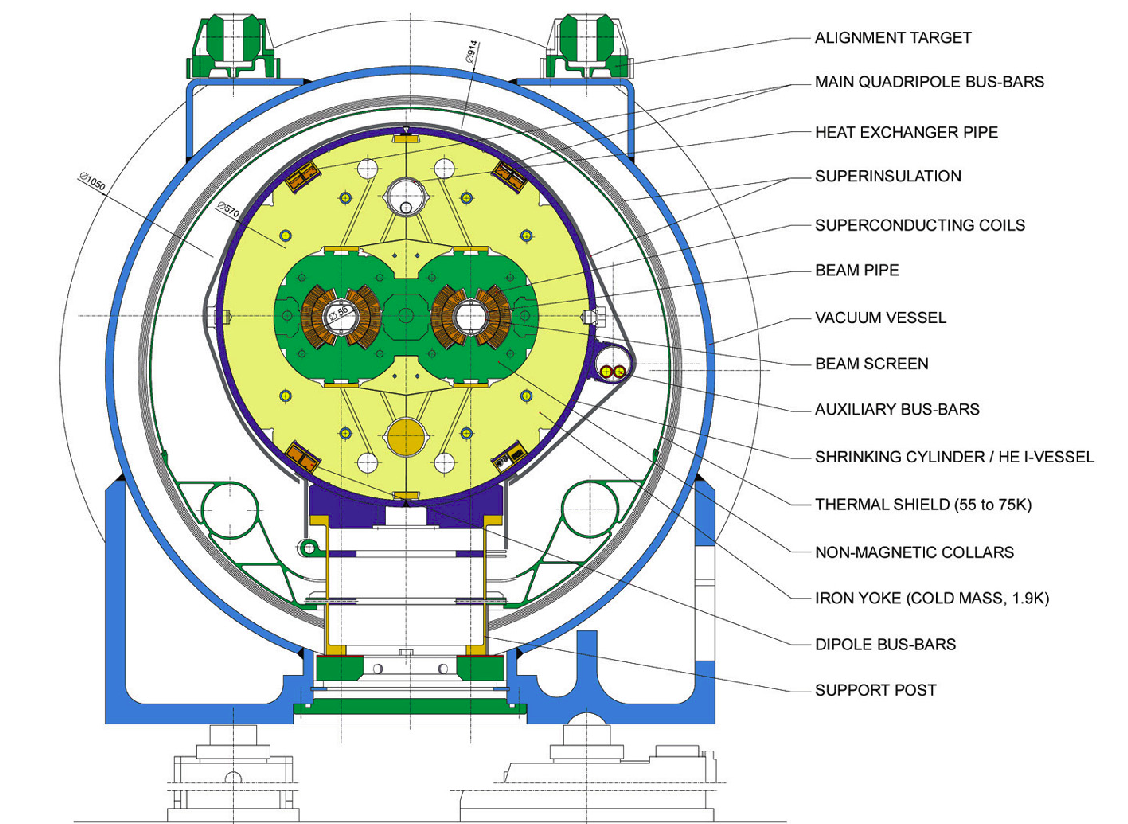
\includegraphics[scale=0.16]{dipole_magnet.png}}
\subfloat[][]{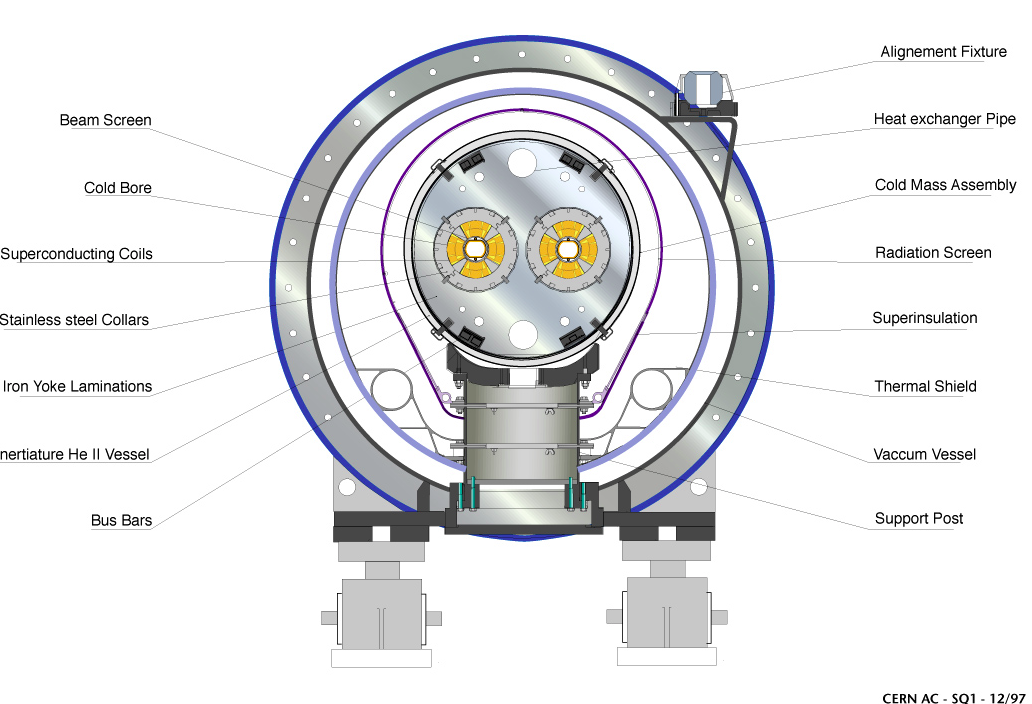
\includegraphics[scale=0.2]{quadrupole_magnet.png}}
\caption{a)Cross-section of the LHC dipole magnets, b)Cross-section of the LHC quadrupole magnets.}
\end{figure}
\\Checking the performaces of the collider, the main parameter to take into account is the instantaneous luminosity, which gives the rate of expected events of a process, once the cross section is known\footnote{The LHC nominal luminosity is $\mathcal{L} = 10^{34}\text{cm}^{-1}\text{s}^{-1}$, involving around one billion proton interactions per second.}
\begin{equation}
\frac{\text{d}N_{process}}{\text{d}t} = \mathcal{L}\sigma_{process}
\end{equation}
where $\sigma_{process}$ is the inelastic proton-proton cross section and
\begin{equation}
\mathcal{L} = f \frac{n_1n_2}{4\pi \sigma_x\sigma_y}
\end{equation}
where $f$ is the bunch crossing frequency, $n_1$ and $n_2$ are the numbers of particles in each bunch and $\sigma_x$ and $\sigma_y$ are the beam widths in the transverse plane.
Going more into LHC details, it can collide bunches of protons with a bunch crossing frequency of 40 MHz, each of them focused to reach down to 15 $\mu\text{m}$ in the transverse plane\cite{Bruning}. Integrating the instantaneous luminosity over a time period, you can find the integrated luminosity
\begin{equation}
L = \int\mathcal{L}dt
\end{equation}
\begin{table}[htb]
\caption{Design and 2016 LHC technical running conditions for proton-proton collisions \cite{LHC_parameters}.}
\centering 
\begin{tabular}{l l}
\hline\hline
\textbf{Parameters} & \textbf{Values} \\ [0.5ex]
\hline
Beam energy at LHC injection & 450 GeV \\
Design beam energy at collision & 7 TeV \\
2016 beam energy at collision & 6.5 TeV \\ [0.5ex]
\hline
Peak magnetic dipole field & 8.33 T \\
Dipole operating temperature & 1.9 K \\ [0.5ex]
\hline
Design instantaneous luminosity & $10^{34} \text{cm}^{-1}\text{s}^{-1}$ \\
2015-18 instantaneous luminosity & $1.2 \cdot 10^{34} \text{cm}^{-1}\text{s}^{-1}$ \\ [0.5ex]
\hline
No. of bunches per proton beam & 2808 \\
No. of proton per bunch (at start) & $1,15 \cdot 10^{11}$ \\
Bunch spacing & 25 ns \\
Minimum distance between bunches & $\sim 7 \text{m}$ \\ [0.5ex]
\hline
Beam lifetime & 10 h \\
Average collision rate & 36.1 MHz \\
Number of collision per second & 600 millions \\ [0.5ex]
\hline\hline
\end{tabular}
\end{table}
\\Tipically the luminosity is not constant during the data taking, but it is subject to decrease as the time goes on. This behaviour is due in particular to the degradation of the intensity of the beam, as a result of proton-proton collisions in the LHC interaction points.  Said that, the luminosity of the collider, seen as a function of time, is
\begin{equation}
\mathcal{L}(t) = \frac{\mathcal{L}_0}{(1+t/\tau_{nuclear})^2}
\end{equation}
with
\begin{equation}
\tau_{nuclear} = \frac{N_{tot,0}}{\mathcal{L}_0\sigma_{tot}k}
\end{equation}
\begin{figure}[htb]
\centering
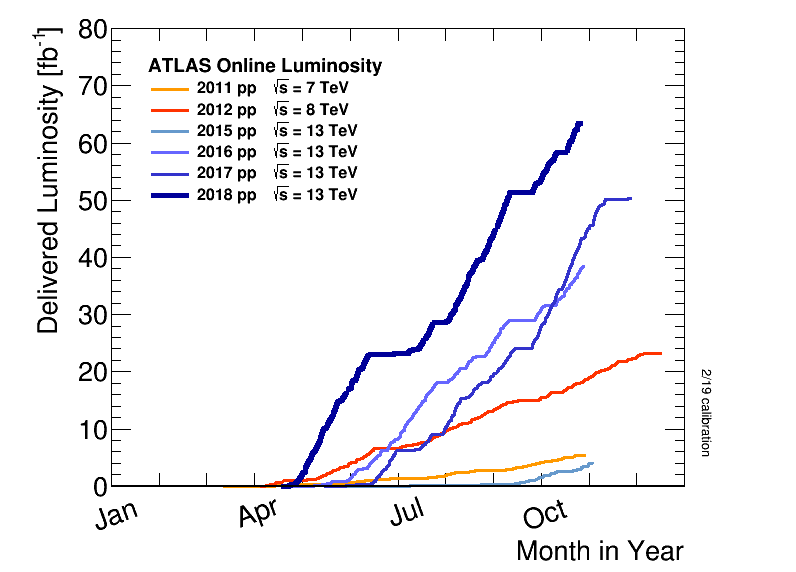
\includegraphics[scale=0.28]{luminosity.png}
\caption{Cumulative luminosity versus day delivered to ATLAS during stable beams and for high energy proton-proton collisions.}
\end{figure}
where $N_{tot,0}$ is the initial beam intensity, $\mathcal{L}_0$ is the initial luminosity at the beam injection $\sigma_{tot}$ stands for the total $pp$ cross section and $k$ is the number of interaction points\footnote{Around the main LHC ring, four different experiments are placed: ATLAS, CMS, LHCb and ALICE. The beams collide into each of these experiments, so at LHC four interaction points are present.}.
\\
In high-luminosity colliders, such as LHC, there is a considerable probability that a single bunch collision may produce several separate events, uncorrelated from the main interaction vertex and deriving usually from soft scattering processes: these kinds of event are known as \emph{pileup} events and are considered as background. The pileup events are strongly related to the instantaneous luminosity and affect the objects reconstruction, making the identification of vertices and tracks more difficult because of the increasing in the number of hits in each collision.
\\
The connection that tie the pileup events rate and the instantaneous luminosity is
\begin{equation}
\mathcal{L} = \frac{\text{rate}_{inelastic}}{\sigma_{inelastic}} = \frac{\mu n_b f_{rev}}{\sigma_{inelastic}}
\end{equation}
where $\mu$ is the number of inelastic interactions per bunch crossing and $n_b$ is the number of colliding bunches in the accelerator. The number of pileup events per bunch crossing is proportional to $\mathcal{L}/f$ and it increases with the instantaneous luminosity.
\begin{figure}[h]
\centering
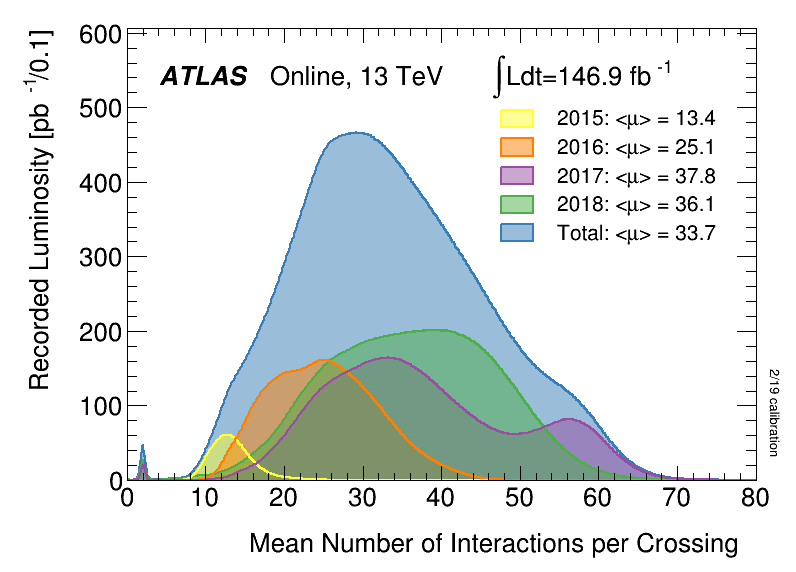
\includegraphics[scale=0.28]{pileup_events.png}
\caption{The luminosity-weighted distribution of the mean number of interactions per crossing for the 2018 pp collision data at 13 TeV centre-of-mass energy.}
\end{figure}


\section{Hadron colliders kinematics}
Because of the fact that hadron colliders run in the relativistic regime, the center-of-mass energy is generally boosted along the beam direction. To describe these kinds of events, a set on kinematic variables invariant under Lorentz boosts in that direction must be used.
A convenient set of these variables is the transverse momentum $p_T$, the  pseudo-rapidity $\eta$ or rapidity $y$ in the limit of a particle is travelling close to the speed of light and the azimuthal angle $\phi$. Using them to redefine the four-momentum $p^{\mu}$ of a particle of mass $m$, this can be written as
\begin{equation}
p^{\mu} = (E, p_x, p_y, p_z) = (m_T\cosh y, p_T\sin\phi, p_T\cos\phi, m_T\sinh y)
\end{equation}
where $p_x$, $p_y$ and $p_z$ are the spatial components of the momentum\footnote{In the third component $p_z$ of the momentum $\vec{p}$ of the particle is directed along the beam direction, while $p_x$ and $p_y$ lie in the transverse $(x,y)$ plane, perpendicular to the beam direction. The $x$ direction points toward the center of the LHC ring and the $y$ direction aims up from the $(z,x)$ plane.}
and the transverse mass $m_T$ is defined as $m_T = \sqrt{p_T^2 + m^2}$.
\\
The pseudo-rapidity $\eta$ describes the angle of a particle relative to the beam axis and it is defined as
\begin{equation}
\eta = -\ln\Bigl[\tan\Bigl(\frac{\theta}{2}\Bigr)\Bigr]
\end{equation}
where $\theta$ is the angle between the particle momentum $\vec{p}$ and the positive $z$ axis. Expressing $\eta$ in terms of the momentum $\vec{p}$, turns out to be
\begin{equation}
\eta = \frac{1}{2}\ln\Bigl(\frac{|\vec{p}| + p_L}{|\vec{p}| - p_L}\Bigr)
\end{equation}
where $p_L$ stands for the component of the momentum along the beam axis.
\\\\
In the limit of very high-energiy particles\footnote{In this limit, the particle's only energy is its momentum-energy, similar to the case of photons.}
, namely when the mass of the particle is negligible and so $m \ll |\vec{p}| \Rightarrow E \approx |\vec{p}|$, the pseudo-rapidity can be reasonably approximated with the definition of rapidity $y$
\begin{equation}
y = \frac{1}{2}\ln\Bigl(\frac{E + p_L}{E - p_L}\Bigr) \hspace{0.4cm} \text{.}
\end{equation}
Notice how the rapidity $y$ is not invariant under Lorent's boosts along the beam direction, but it transforms such as
\begin{equation}
y \longrightarrow y + \frac{1}{2}\ln\Bigl(\frac{1 + \beta}{1 - \beta}\Bigr)
\end{equation}
where $\beta$ is the boost velocity.
\\
Another common variable used to parametrise the angular separation between particles produced in an hadron collision is $\Delta R$, which is defined as
\begin{equation}
\Delta R = \sqrt{(\Delta\eta)^2 + (\Delta\phi)^2}
\end{equation}
where $\Delta\eta$ and $\Delta\phi$ are the differences in the $\eta$ and $\phi$ coordinates for the particles, respectively.